	\chapter{METHODOLOGY}
	\label{chap:work}
	
	\section{Vehicle Classification}
	
	 Electric vehicles have been classified primarily into four major categories as shown in Figure~\ref{fig:classification} 
	 	
			\begin{figure}[h]
				\centering
				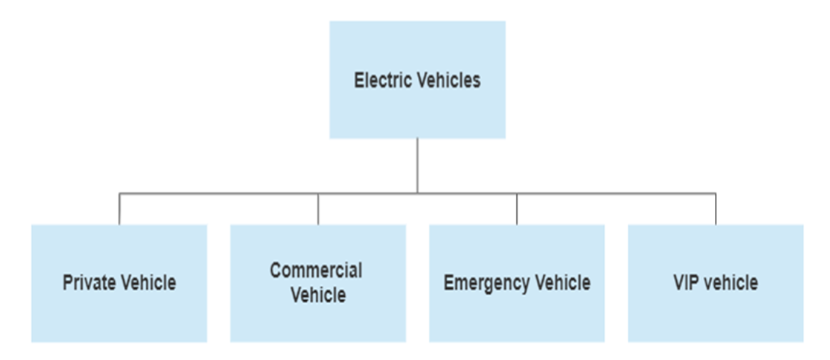
\includegraphics[width=0.7\linewidth]{classification}
				\caption{Vehicle Classification}
				\label{fig:classification}
			\end{figure}
		
	The above classification is made by comparing the battery capacity of the vehicles from the data \cite{evdata} taken with the battery capacity of the similar kind of vehicles in the market.

	\par {Private vehicles are further classified into E-bikes and E-cars with average battery capacity of 400Wh to 500 Wh and 40 kWh to 100 Kwh respectively. Commercial vehicles are classified into E-Truck and E-Bus with an average battery capacity of 100 KWh and 60 to 548 KWh respectively. Emergency vehicles have a battery capacity of around 105 KWh and VIP vehicles have around 90 KWh to 200 KWh.
	}
	
	\section{Travel Pattern Establishment}
	
	Travel pattern for three main vehicle subcategories of the above mentioned vehicle categories namely E-car, E-Truck and E-Bus are now taken and travel patterns of the same have been established by using the Battery capacity, Time taken to full charge, Time period of the vehicle when it is connected to the grid , charging rate and discharging rate\cite{evdata}.
	
<<<<<<< HEAD
	\section{Charging/Discharging Pattern}
	
	\section{Proposed Algorithm}
		\begin{figure}
			\centering
			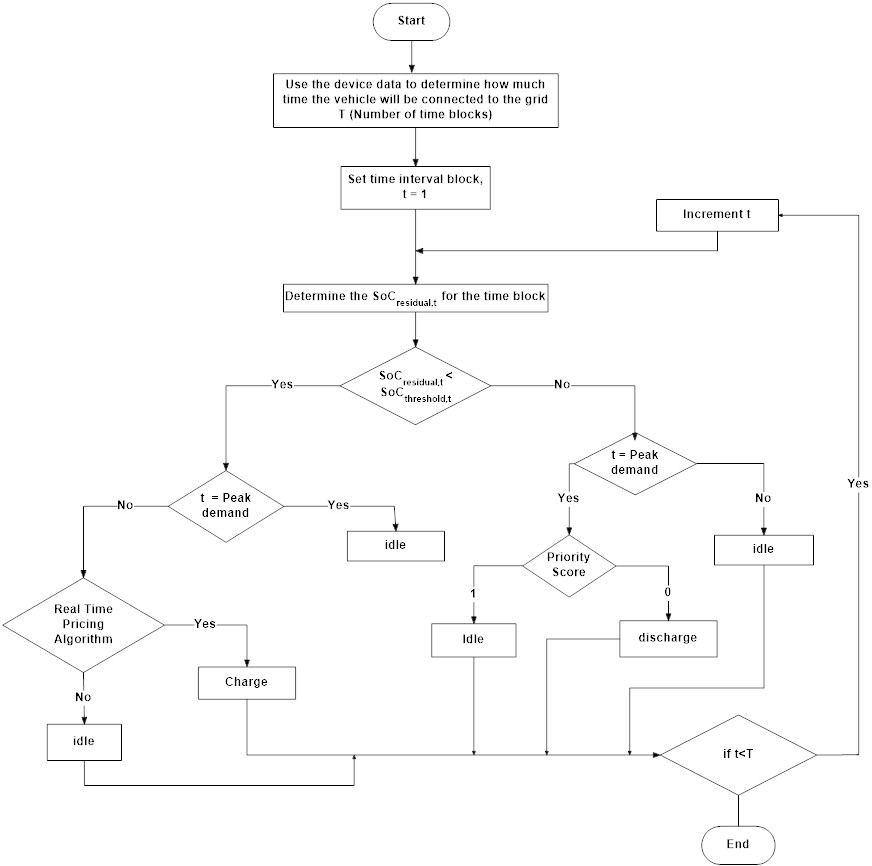
\includegraphics[width=1\linewidth]{Ev_flowchart}
			\caption{Proposed Algorithm for determining Charging/Discharging Pattern}
			\label{fig:evflowchart}
		\end{figure}
		
	
	
=======
	\section{Charging/Discharging pattern Establishment}
>>>>>>> da5d510a18713a0bf36cffc1bc12cfc95bf4234c
